% Copyright © 2012-2013 Martin Ueding <dev@martin-ueding.de>
%
\input{header.tex}

\usepackage{float}
\usepackage{scrpage2}
\usepackage{tikz}
\usetikzlibrary{calc}

\newcommand{\themodul}{physik311}
\newcommand{\thegruppe}{Gruppe 3 -- Matthias Rehberger}
\newcommand{\theuebung}{12}

\pagestyle{scrheadings}

\cfoot{\footnotesize{\thegruppe}}
\ifoot{\footnotesize{Martin Ueding}}
\ofoot{\footnotesize{Seite \thepage\ / \pageref{LastPage}}}
\ihead{\themodul{} -- Übung \theuebung}
\ohead{\rightmark}
\chead{}
\setheadsepline{.4pt}
\automark{section}

\setcounter{section}{39}


\def\thesubsection{\thesection\alph{subsection}}

\title{\themodul{} -- Übung \theuebung \\ \vspace{0.5cm} \large{\thegruppe}}

\author{Martin Ueding \\ \small{\href{mailto:mu@uni-bonn.de}{mu@uni-bonn.de}}}

\begin{document}

\maketitle

\begin{table}[h]
	\centering
	\begin{tabular}{l|c|c|c|c|c|c}
		Aufgabe
		& \ref 1
		& \ref 2
		& \ref 3
		& \ref 4
		& \ref 5
		& $\sum$ \\
		\hline
		Punkte
		& \punkte
		& \punkte
		& \punkte
		& \punkte
		& \punkte
	\end{tabular}
\end{table}

%%%%%%%%%%%%%%%%%%%%%%%%%%%%%%%%%%%%%%%%%%%%%%%%%%%%%%%%%%%%%%%%%%%%%%%%%%%%%%%
%                               Doppelbrechung                                %
%%%%%%%%%%%%%%%%%%%%%%%%%%%%%%%%%%%%%%%%%%%%%%%%%%%%%%%%%%%%%%%%%%%%%%%%%%%%%%%

\section{Doppelbrechung}
\label 1

\begin{figure}
	\centering
	\includegraphics{40_cropped.pdf}
	\caption{Konstruktion für einen einachsig-positiven Kristall}
	\label{fig:1}
\end{figure}

Die Beugung von außerordentlichem Licht im einachsig-positiven Kristall ist in
Abbildung \ref{fig:1} dargestellt. Dabei wird das ordentliche Licht nicht
gebeugt, da sich das Medium isotrop verhält. Für das außerordnetliche Licht
sind die Huygens-Kugelwellen Ellipsoide, so dass der Lichtstrahl abgelenkt
wird. Dabei wird er von der optischen Achse weg gebeugt. Falls der Kristall
einachsig-positiv ist, würde das Licht in die andere Richtung, also zur
optischen Achse, gebeugt.

%%%%%%%%%%%%%%%%%%%%%%%%%%%%%%%%%%%%%%%%%%%%%%%%%%%%%%%%%%%%%%%%%%%%%%%%%%%%%%%
%                      Doppelbrechung und Faraday-Effekt                      %
%%%%%%%%%%%%%%%%%%%%%%%%%%%%%%%%%%%%%%%%%%%%%%%%%%%%%%%%%%%%%%%%%%%%%%%%%%%%%%%

\section{Doppelbrechung und Faraday-Effekt}
\label 2

Das $\lambda/2$-Plättchen kehrt die Amplitude des außerordentlichen Lichts um,
die Amplitude des ordentlichen Lichts bleibt allerdings gleich. Dies entspricht
einer Spiegelung der Polarisationsrichtung. Bei zweimaliger Anwendung wird das
Licht wieder in die ursprüngliche Richtung gelenkt. Die Ablenkung um
$\unit{\pi/4}\radian$ erfordert, dass die Hauptachse und Polarisationsrichtung
vorher um $\unit{\pi/8}\radian$ zueinander verdreht waren.

Bei der Faraday-Zelle hängt die Drehung der Polarisationsrichtung nicht von der
Durchlaufrichtung ab. Die Drehungen werden so addiert. Nach zwei Durchläufen
hat sich die Polarisationsrichtung um $\unit{\pi/2}\radian$ gedreht.

%%%%%%%%%%%%%%%%%%%%%%%%%%%%%%%%%%%%%%%%%%%%%%%%%%%%%%%%%%%%%%%%%%%%%%%%%%%%%%%
%                              Wollaston-Prisma                               %
%%%%%%%%%%%%%%%%%%%%%%%%%%%%%%%%%%%%%%%%%%%%%%%%%%%%%%%%%%%%%%%%%%%%%%%%%%%%%%%

\section{Wollaston-Prisma}
\label 3

Das einfallende Licht kann in einen ordentlichen und außerordentlichen Anteil
aufgespalten werden (lineare Superposition). Da die optische Achse allerdings
parallel zur Grenzfläche ist und die Strahlen senkrecht zur Grenzfläche
eintreten, tritt keine Ablenkung ein. Die Phasenverschiebung durch die
Verzögerung sollte keinen Effekt haben, da das Licht nicht unbedingt vorher
kohärent war.

An der Grenzfläche zwischen den beiden Teilen tauschen die
Polarisationsrichtungen die Rollen. Der bisher ordentliche Teil wird nun
abgelenkt. Der vorher außerordentliche Teil wird nun zum ordentlichen.

Dies bedeutet, dass sich die Ausbreitungsgeschwindigkeit ändert. Sinnvollerweise hat Quarz nicht einen, sondern zwei Brechungsindizes: $n_\text{o}$ und $n_\text{ao}$. Mit dem normalen Brechungsgesetz erhalte ich folgende Relationen:
\[
	\frac{\sin\del{\alpha}}{\sin\del{\beta_\text{o}}}
	= \frac{n_\text{ao}}{n_\text{o}}
	\eqnsep
	\frac{\sin\del{\alpha}}{\sin\del{\beta_\text{ao}}}
	= \frac{n_\text{o}}{n_\text{ao}}
\]

Dabei bezeichnet $\alpha$ den Keilwinkel ($\alpha = 15\degree$),
$\beta_\text{o}$ den Winkel zwischen dem \emph{zu Anfang} ordentlichen Strahls
und der Trennflächennormale.

Mit $n_\text{o} = 1.544$ und $n_\text{ao} = 1.553$\footnote{\url{https://en.wikipedia.org/wiki/Birefringence\#Examples\_of\_uniaxial\_birefringent\_materials}} erhalte ich:
\[
	\beta_\text{o} = \unit{0.260247}\radian
	\eqnsep
	\beta_\text{ao} = \unit{0.263362}\radian
\]

An dieser Stelle habe ich also $\Delta \beta = \unit{3.11}{\milli\radian}$.

Danach müssen beide Strahlen noch das Prisma verlassen, so dass erneut ein
Übergang entsteht, diesmal zur Luft. Die Normale der Rückseite steht noch um
$\alpha$ zur der Trennflächennormale. Ich bilde neue Winkel $\gamma = \beta -
\alpha$.  Für die Austrittswinkel $\delta$ zur Normale der Rückseite gilt
wieder das Brechungsgesetz:
\[
	\frac{\sin\del{\gamma_\text{o}}}{\sin\del{\delta_\text{o}}}
	= \frac{1}{n_\text{ao}}
	\eqnsep
	\frac{\sin\del{\gamma_\text{ao}}}{\sin\del{\delta_\text{ao}}}
	= \frac{1}{n_\text{o}}
\]

Für $\delta$ erhalte ich:
\[
	\delta_\text{o} = \unit{-2.41104}{\milli\radian}
	\eqnsep
	\delta_\text{ao} = \unit{2.41205}{\milli\radian}
\]

Der Winkel zwischen den beiden Strahlen beträgt $\Delta \delta =
\unit{4.82309}{\milli\radian}$.

Beim Glan-Foucault Prisma ist in der Mitte ein Luftspalt, so dass
Totalreflexion eintritt. Auf diese Weise bleibt im geraden Durchgang nur noch
eine Polarisation übrig, alles andere wurde reflektiert.

%%%%%%%%%%%%%%%%%%%%%%%%%%%%%%%%%%%%%%%%%%%%%%%%%%%%%%%%%%%%%%%%%%%%%%%%%%%%%%%
%                               Compton-Effekt                                %
%%%%%%%%%%%%%%%%%%%%%%%%%%%%%%%%%%%%%%%%%%%%%%%%%%%%%%%%%%%%%%%%%%%%%%%%%%%%%%%

\section{Compton-Effekt}
\label 4

Es handelt sich um einen elastischen Stoß, somit muss die Energie, die dem Photon entzogen wird, komplett auf das Elektron übertragen werden:
\[
	hf - hf' = E_\text{kin}
\]

Für die Impulserhaltung nehme ich an, dass der Impuls des Photons nur wenig kleiner wird. Aus Abbildung \ref{fig:3}, in der $hf/c$ und $hf'c$ gleich lang sind, kann ich ablesen, dass gilt:
\[
	m_e v = \frac{hf}c \sin\del{\frac \theta 2}
\]

\begin{figure}
	\centering
	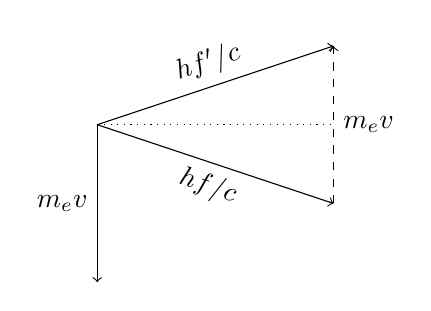
\begin{tikzpicture}
		\coordinate (o) at (0, 0);
		\coordinate (a) at (3, -1);
		\coordinate (b) at (3, 1);
		\coordinate (c) at (0, -2);

		\draw[->] (o) -- (a) node[below, midway, sloped] {$hf/c$};
		\draw[->] (o) -- (b) node[above, midway, sloped] {$hf'/c$};
		\draw[->] (o) -- (c) node[left, midway] {$m_e v$};
		\draw[dashed, ->] (a) -- (b) node[right, midway] {$m_e v$};
		\draw[dotted] (o) -- ($(a)!.5!(b)$);
	\end{tikzpicture}
	\caption{Skizze zum Compton-Effekt}
	\label{fig:3}
\end{figure}

Die beiden Relationen kann ich umformen und gleichsetzen:
\begin{align*}
	E_\text{kin}
	= \half m_e v^2
	= \frac{(m_ev)^2}{2m_e}
	= \frac{4h^2f^2}{2m_ec^2} \sin^2\del{\frac \theta 2}
	&= hf - hf'
	&&\left| \div hf^2 \right. \\
	%
	\frac{4h}{2m_ec^2} \sin^2\del{\frac \theta 2}
	&= \frac{f - f'}{f^2}
	\approx \frac{1}{f'} - \frac{1}{f}
	&&\left| \frac 1f = \frac \lambda c \right. \\
	%
	\frac{2h}{m_ec} \sin^2\del{\frac \theta 2}
	&= \lambda' - \lambda
\end{align*}

%%%%%%%%%%%%%%%%%%%%%%%%%%%%%%%%%%%%%%%%%%%%%%%%%%%%%%%%%%%%%%%%%%%%%%%%%%%%%%%
%                      Absorption in einer Rubidiumzelle                      %
%%%%%%%%%%%%%%%%%%%%%%%%%%%%%%%%%%%%%%%%%%%%%%%%%%%%%%%%%%%%%%%%%%%%%%%%%%%%%%%

\section{Absorption in einer Rubidiumzelle}
\label 5

Ich benutze die ideale Gasgleichung um Druck $P$ und Temperatur $T$ in eine
Atomdichte pro Fläche erhalten. Dazu benutze ich die Länge $l$ der Kammer und
ihre Querschnittsfläche $F$ sowie dass die Stoffmenge $n$ (in \mole) und die
Teilchenzahl $n$ sich verhalten wie $n N_A = N$:
\[
	PV = NRT
	\iff
	PlF = NRT
	\iff
	\frac NF = \frac{Pl}{RT}
\]

Dies multipliziere ich mit dem gegebenen Wirkungsquerschnitt $\sigma =
\lambda^2/(2 \pi)$ um den Anteil der Fläche zu bekommen, die mit Atomen
versperrt ist. Dabei setze ich auch ein, dass gemittelt nur ein von
hundert Atomen ein Photon absorbiert. Dies gibt dann den
Absorptionsfaktor $k$:
\[
	k := \frac{n \sigma}{100 F}
\]

Ich setze die Zahlen ein. $P = \unit{10^{-4}}\pascal$, $l =
\unit{5 \e{-2}}\meter$, $T = \unit{300}\kelvin$, $\lambda =
\unit{780^{-9}}\meter$, $R = 8.31446$:
\[
	\frac nF = \unit{2.41\e{14}}{\meter\rpsquared}
	\eqnsep
	k = \frac{P l \lambda^2}{200 \pi R T} = 1.90 \e{-6}
\]

Mit $\sigma = \pi \cdot \unit{25\e{-20}}{\meter\squared}$ erhalte ich exakt den gleichen Wert.

Wenn der Resonator um das Gas perfekt wäre, würde es in der Größenordnung
$500000$ Durchläufe benötigen, bis die Zahl auf $1/\ee$ abgefallen ist. Dies
entspricht einer Relaxationszeit von $\tau = \unit{17}{\micro\second}$. Das Gas
hat also durchaus einen Effekt auf das Licht.

%\bibliography{../../zentrale_BibTeX/Central}
%\bibliographystyle{plain}

\end{document}

% vim: spell spelllang=de
